\chapter[Activation Functions]{Activation Functions}
\label{ch:activation-functions}\index{activation functions|(}
``Neural networks were originally conceived as a model that would imitate the function of the human brain---a set of neurons joined together by a set of connections. Neurons, in this context, are composed of a weighted sum of their inputs followed by a nonlinear function, which is also known as an activation function.''\cite{caterini2018}

Activation Functions are used in Artificial Neural Networks to determine whether the output of the neuron should be considered further or ignored. If the activation function chooses to continue considering the output of a neuron, we say that the neuron has been activated. The output of the activation function is what is passed on to the subsequent layer in a multilayer neural network. To determine whether a neuron should be activated, the activation function takes the output of a neuron and transforms it into a value commonly bound to a specific range, typically from $0$ to $1$ or $-1$ to $1$ depending on the which activation function is applied.

\section{Step Function}\label{sec:step-function}\index{step function}
\begin{figure}
  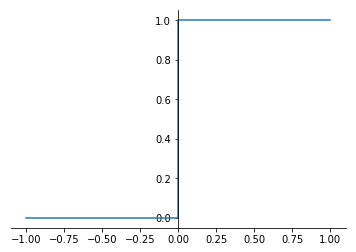
\includegraphics{graphics/activation_functions/step_function.png}
  \label{fig:stepfunction}
  \caption{
    A graph of the step function which is defined by: 
    $$
      f(x) =
      \begin{dcases*}
                                       0 & \text{for \(x < 0\)} \\
                                       1 & \text{for \(x \geq 0\)} \\
      \end{dcases*}
    $$
    
    The derivative of the step function is:
    $$
      \frac{d}{d(x)}f(x) =
      \begin{dcases*}
                                       0 & \text{for \(x \neq 0\)} \\
                                       ? & \text{for \(x = 0\)} \\
      \end{dcases*}
    $$
  }
\end{figure}
The Heavside step function, also known as binary step function, is one of the simplest activation functions that can be used in a neural network. This activation function returns $0$ if the input of a node is less than a predetermined threshold (typically $0$), or otherwise it returns $1$ if the output of the node is greater than or equal to the threshold. This function was first used in a machine learning context in 1957 by Frank Rosenblatt in his seminal work describing the perceptron, the precursor to the modern day neural network\cite{rosenblatt1957perceptron}. 

Nowadays, the step function is seldom used in practice as it cannot be used to classify more than one class. Furthermore, since the derivative of this function is $0$, gradient descent algorithms are not be able to progressively update the weights of a network that makes use of this function\cite{Snyman2005}.

\section{Linear Functions}\label{sec:linear-function}\index{linear activation function}
A linear activation function seeks to solve some of the shortcomings of the step function. The output produced by a linear activation function is proportional to the input. While a linear activation function could be used for multi-class problems, it can on be used on problems that are linearly separable. Linear functions can also run into problems with gradient descent algorithms, as the derivative of a linear function is a constant. Additionally, since the output of the linear function is not bound to any range, it could be susceptible to a common problem when training deep neural networks called the exploding gradient problem, which can make learning unstable\cite{goodfellow2016deeplearning}.

\section{Sigmoid and Hyperbolic Tangent}\label{sec:sigmoid-tanh}\index{sigmoid function}\index{hyperbolic tangent}

\begin{figure}
  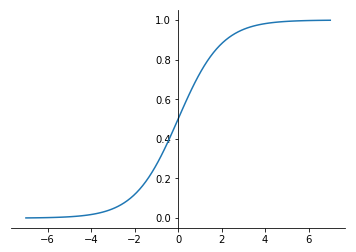
\includegraphics{graphics/activation_functions/sigmoid_function.png}
  \label{fig:sigmoidfunction}
  \caption{
    A graph of the sigmoid function which is defined by:
    $$
    f(x) = \frac{1}{(1 + e^{-x})}
    $$
    
    The derivative of the sigmoid function is:
    $$
    \frac{d}{d(x)}f(x) = f(x)(1-f(x)).
    $$
  }
\end{figure}
The sigmoid function, also known as the logistic function, is one of the most commonly used activation functions in neural networks, because of its simplicity and desirable properties. The use of this function in neural networks was first introduced by Rummelhart, Hinton and Williams in one of the most important papers in the field of machine learning, which described the back-propagation algorithm and the introduction of hidden layers, giving rise to modern day neural networks\cite{DavidE.Rumelhart1986Lrbb}.  The values produced by the step function are bound between $0$ and $1$, both not inclusive, which help manage the exploding gradient problem. The function also has a very steep gradient for a relatively small range of values, typically in the range of $-2$ to $2$. This means that for most inputs that the function receives it will return values that are very close to either $0$ or $1$.

On the other hand, this last property makes the sigmoid function very susceptible to the vanishing gradient problem\cite{bengio94}. When observing the shape of the sigmoid function we see that towards the ends of the curve, function becomes very unresponsive to changes in the input. In other words, the gradient of the function for large inputs becomes very close to $0$. 

\begin{figure}
  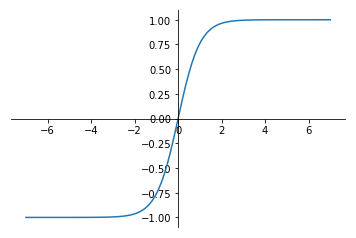
\includegraphics{graphics/activation_functions/tanh_function.png}
  \label{fig:tanhfunction}
  \caption{
    A graph of the hyperbolic tangent ($tanh$) function which is defined by:
    $$
    f(x) = tanh(x) = \frac{e^x - e^{-x}}{(e^x + e^{-x})}
    $$
    
    The derivative of the $tanh$ function is:
    $$
    \frac{d}{d(x)}f(x) = 1-f(x)^2.
    $$
  }
\end{figure}
The hyperbolic tangent ($tanh$) function is another activation function that is sometimes used instead of sigmoid. The $tanh$ function has the same characteristics of the sigmoid function mentioned above. In fact if one plots the $tanh$ function, one can observe that it is simply a scaled version of the sigmoid function. As a result of this scaling, the tanh function has a steeper gradient in towards the origin, and it returns values between $-1$ and $1$.

Nowadays with the rise of deep learning, these functions are becoming less commonly used. Xavier Glorot and Yoshua Bengio studied in detail the effects of the sigmoid and tanh activation functions. They note how the sigmoid function in particular is not well suited for deep networks with random initialization\cite{glorot2010understanding}.

\section{Rectified Linear Unit}\label{sec:relu}\index{rectified linear unit (relu)}
\begin{figure}
  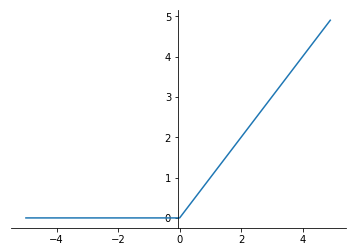
\includegraphics{graphics/activation_functions/relu_function.png}
  \label{fig:relufunction}
  \caption{
    A graph of the ReLU function which is defined by:
    $$
      f(x) =
      \begin{dcases*}
                                       0 & \text{for $x < 0$} \\
                                       x & \text{for $x \geq 0$} \\
      \end{dcases*}
    $$
    
    The derivative of the ReLU function is:
    $$
      \frac{d}{d(x)}f(x) =
      \begin{dcases*}
                                       0 & \text{for $x < 0$} \\
                                       1 & \text{for $x \geq 0$} \\
      \end{dcases*}
    $$
  }
\end{figure}
The ReLU function returns $0$ if the input of the function is negative, otherwise it outputs the value of the input itself. This function is non-linear in nature even though at first glance it may seem similar to an identity function. The ReLU function is becoming one of the more commonly used activation function due to its simplicity performance, and suitability to networks with many layers. Another benefit of the ReLU function is that it produces sparse activations (not all nodes in the network are activated) unlike the sigmoid or hyperbolic tangent functions. 

The ReLU function has been used in many neural network models to improve their performance. Naid and Hinton use ReLU to improve the performance of Restricted Boltzmann Machines in object recognition\cite{Nair2010}. In 2012, a breakthrough Convolutional Neural Network (CNN) architecture called AlexNet pioneered the use of the ReLU activation function together with dropout layers to minimise over fitting in CNNs.\cite{KrizhevskyAlex2017Icwd}. 

Unfortunately, because the gradient of the function for inputs that are negative is $0$, the ReLU function can still be susceptible to the vanishing gradient problem. To manage this problem a variant of the ReLU function, called Leaky ReLU is sometimes used. Rather than simply returning 0 for negative inputs, the leaky ReLU return a very small value such as $0.01x$. However, researchers at the University of Stanford compared the performance of Sigmoid, ReLU and Leaky ReLU functions and found that while the the performance of both the ReLU and Leaky Relu functions was better than the performance achieved with the sigmoid function, the performance of the two ReLU functions was nearly identical\cite{maas2013rectifier}.
\index{activation functions|)}
